\chapter{Evaluation}

\section{\bb 3 alignment benchmark dataset}
\begin{wrapfigure}{r}{0.4\textwidth}
	\centering
	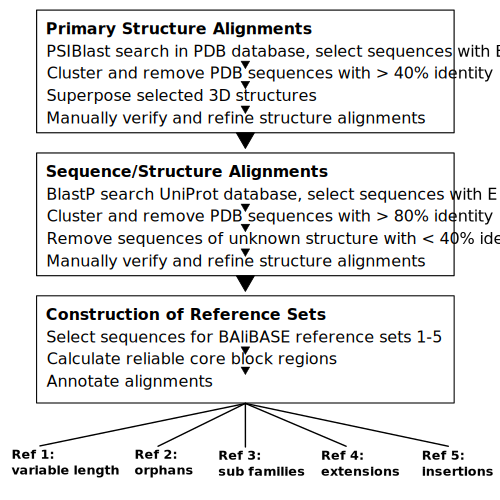
\includegraphics[width=0.5\textwidth]{./images/balibase.png}
	\caption{Flow chart showing the semi automatic process used to establish the reference sets TODO cite self}
	\label{fig:balibase}
\end{wrapfigure}

The third version of the \bb benchmark protein alignment database has been released in 2005 and is widely employed for the comparison of multiple alignment programs \cite{thompson2005balibase, Russell2016}. It is constructed in a semi automatic process as shown in \cref{fig:balibase} and suitable to evaluate global and local alignment programs. The database is split into 5 reference sets with different characteristics representing distinctive multiple alignment problems. \\
It is divided into:



\begin{itemize}
	\item reference set 1 subset V1, for which any two sequences share <20\% identity and no internal insertions over 35 residues long
	\item reference set 1 subset V2, consisting of families with at least four equidistant sequences for which any two sequences share 20-40\% identity and no large insertions
	\item reference set 2, for which all sequences share >40\% identity and at least one 3D structure is known. Additionally an "Orphan" sequence with <20\% identity is chosen per family
	\item for reference set 3, all sequences in the same subfamily have >40\% identity, whereas sequences from different subfamilies share <20\% identity
	\item for reference sets 4 and 5, every sequence shares at least 20\% with one other sequence, including sequences with large N/C-terminal extensions (ref 4) or internal insertions (ref 5)
\end{itemize}

\subsection{Core blocks}

Evaluating and comparing alignment programs is a difficult problem due to the uncertainty of supposedly "real" alignments of actual sequences. The \bb database  marks alignment columns which can be reliably aligned as so called "core blocks". These core blocks are calculated and manually verified, making up 19\% of the full length sequences which are used in the evaluation of \textit{spam-align} \cite{thompson2005balibase}.

%\begin{itemize}
%	\item what are core blocks?
%	\item how are they determined and validated?
%\end{itemize}

\begin{figure}[h]
	\centering
	\includegraphics[width=0.8\textwidth]{./images/balibase-web.png}
	\caption{\bb web interface. Black columns indicate core blocks. \href{www.lbgi.fr/wscoperr?Balibase&FileMoi&macsimHtml&BB20006}{lbgi.fr}}
	\label{}
\end{figure}


\section{Sum-of-pairs and column score}
Comparing the alignment output of different methods can be done by computing the sum-of-pairs and column scores.\\
Given a test alignment $A_t$ and a reference alignment $A_r$ with $M$ sequences and $N_t, N_r$ columns respectively, the sum-of-pairs and column score is defined according to Thompson et al. \cite{thompson1999comprehensive}.

\begin{mydef}[Sum-of-pairs score]
	The sum of pairs score is the ratio of correctly aligned individual residues. Formally it is defined as:
	\begin{align*}
		p_{ijk} &= \begin{cases}
		1 \text{ if residues $A_{t{_ij}}$ and $A_{t_{ik}}$ \textbf{are} aligned in $A_r$}\\
		0 \text{ otherwise}
		\end{cases} \\
		S_i &= \sum_{j=1}^{M} \sum_{k=i+1}^{M} p_{ijk} \\
		SPS &= \frac{\sum_{i=1}^{N_t} S_i} {\sum_{i=1}^{N_r} S_{r_i}}
 	\end{align*}
 	with $S_{r_i}$ being the number of correctly aligned residues in the reference.
\end{mydef}

\begin{mydef}[Column score]
	The column score is the ratio of correctly aligned columns. 
	\begin{align*}
	C_i &= \begin{cases}
	1 \text{ if all the residues in the i-th column are aligned correctly}\\
	0 \text{ otherwise}
	\end{cases} \\
	CS &= \frac{\sum_{i=1}^{N_t} C_i}{N_r}
	\end{align*}
\end{mydef}
Note that $C_i = 1$ only if all the residues in the $i$-th column are aligned correctly and no residue belonging to this column is part of another one. For this reason, the numerator is smaller or equal to the denominator.\\
The definition of the column score is slightly different than that provided by the authors of \bb \cite{thompson1999comprehensive} but resembles the actual implementation in the included BaliScore tool and its reimplementation provided with this thesis.\\
These scores are only calculated for the core blocks of the \bb alignments, meaning that for the following evaluation $A_t$ is an alignment over the full sequences, while $A_r$ contains only the aligned residues inside the core blocks.

\section{Evaluated programs}


\subsection{Mafft}
Additionally to \textit{Dialign2.2} and \textit{spam-align} the widely used multiple alignment program \textit{MAFFT} (version 7) is evaluated. It employs a progressive alignment strategy 

\begin{itemize}
	\item progressive alignment
	\item guide tree from all pairwise alignments
\end{itemize}

\subsection{Dialign}

\subsection{Spam}

\section{Results}
